\documentclass[english,11pt]{article}

\pdfoutput=1

\usepackage[T1]{fontenc}
\usepackage[latin9]{inputenc}
\usepackage{verbatim}
\usepackage{float}
\usepackage{amsthm}
\usepackage{amsmath}
\usepackage{amssymb}
\usepackage{graphicx}
%\usepackage{multirow}
\usepackage{color}
\usepackage{url}
\usepackage{caption}
\usepackage{subcaption}
\usepackage{mathtools} 
\usepackage[margin=1.2in]{geometry}

\newcommand{\TODO}[1]{{\color{red}{[#1]}}}

\makeatletter

%%%%%%%%%%%%%%%%%%%%%%%%%%%%%% Textclass specific LaTeX commands.
\numberwithin{equation}{section}
%\numberwithin{figure}{section}
\theoremstyle{plain}
\newtheorem{thm}{\protect\theoremname}[section]
\theoremstyle{definition}
\newtheorem{defn}[thm]{\protect\definitionname}
\theoremstyle{remark}
\newtheorem{claim}[thm]{\protect\claimname}
\theoremstyle{plain}
\newtheorem{lem}[thm]{\protect\lemmaname}

\newtheorem*{lem*}{Lemma}

\theoremstyle{remark}
\newtheorem{rem}[thm]{\protect\remarkname}
\theoremstyle{plain}
\newtheorem{corollary}[thm]{\protect\corollaryname}
\theoremstyle{plain}
\newtheorem{proposition}[thm]{\protect\propositionname}
%%%%%%%%%%%%%%%%%%%%%%%%%%%%%% User specified LaTeX commands.
%\usepackage{slashbox}

\usepackage{babel}
\providecommand{\claimname}{Claim}
\providecommand{\definitionname}{Definition}
\providecommand{\lemmaname}{Lemma}
\providecommand{\remarkname}{Remark}
\providecommand{\theoremname}{Theorem}
\providecommand{\corollaryname}{Corollary}
\providecommand{\propositionname}{Proposition}


\newcommand{\reals}{\mathbb{R}}
\newcommand{\RL}{\mathbb{R}^L}
\newcommand{\CL}{\mathbb{C}^L}
\newcommand{\RN}{\mathbb{R}^N}
\newcommand{\RNN}{\mathbb{R}^{N\times N}}
\newcommand{\CNN}{\mathbb{C}^{N\times N}}
\newcommand{\inner}[1]{\left\langle {#1} \right\rangle}
\newcommand{\hx}{\hat{x}} 
\newcommand{\one}{\mathbf{1}} 
\newcommand{\SNR}{{\textsf{SNR}}} 

\begin{document}

\title{Toward single particle reconstruction without particle picking}


\author{Tamir Bendory, Nicolas Boumal, William Leeb and Amit Singer}
\maketitle

\begin{abstract}
	Here comes the abstract
\end{abstract}

\section{Introduction}

Single particle reconstruction (SPR) using cryo--electron microscopy (cryo--EM) is an innovative technology for reconstructing the 3-D structure of macromolecules. In recent years, structures
of many molecules, previously regarded as insurmountable, are now being reconstructed to near-atomic resolution; see for instance~\cite{kuhlbrandt2014resolution,bartesaghi20152}. This technological advancement was recognized by the 2017 Nobel Prize in Chemistry~\cite{nobel}. 

In a cryo--EM experiment, multiple biological samples of the (ideally) same molecule are rapidly frozen in a thin layer of vitreous ice. Within the ice, the molecules are randomly oriented and positioned. Then, the microscope produces a 2D tomographic projection image, called a \emph{micrograph}, of the multiple samples embedded in the ice. The micrograph is dominated by noise due to the small electron doses that
can be applied to the specimen without causing radiation damage.
The cryo--EM problem is to estimate the structure of the molecule from the micrograph (or, typically, several micrographs). 

\paragraph{Particle picking.}
All contemporary methods in the field split the reconstruction procedure to several subroutines. 
The first step in the pipeline is the so-called \emph{particle picking}, in which one aims to detect the 2D tomographic projections of the samples from the noisy micrograph. The output of ideal particle picker is a series of 2D images, each contains one centered tomographic projection associated with an unknown 3D orientation. This series of images 
is then used to estimate the structure.

Many automatic and semi-automatic methods for particle picking have been proposed, based on edge detection, template matching and deep learning; see for instance~\cite{harauz1989automatic,ogura2004automatic,zhu2016deep,frank1983automatic,scheres2015semi,heimowitz2018apple}. 
However, most of these procedures are prone to \emph{model bias}. For instance, in the popular framework of RELION~\cite{scheres2015semi}, the user manually marks hundreds of spots on the micrograph, believed to contain projections. 
Therefore, the algorithm performance depends on the user prior assumption about the particle's structure; the same holds true for deep learning based approaches which require constructing labeled set of data.
Other methods use disks or difference of Gaussians as templates~\cite{langlois2014automated,voss2009dog}.
Nowadays, it also still popular to pick particles manually. This method, while exploits the researcher's experience, is both tedious and subject to model bias.

The significance of the model bias in cryo--EM was stressed in~\cite{shatsky2009method,henderson2013avoiding} and demonstrated by the ``Einstein from noise'' example.
In this experiment, the image of Einstein is correlated with multiple images of pure noise. The noisy images are then aligned to Einstein's image using cross-correlation and  averaged. 
In~\cite{shatsky2009method}, it was shown that using merely 1000 noise images, the averaged image is remarkably similar to the template image of 
Einstein, rather than to pure noise. 
%Therefore, such a simple algorithm is biased towards its model which is an undesirable property. 
In the context of cryo--EM, this example demonstrates how our prior assumptions about the particle may influence the reconstructed structure.

Besides the model bias, particle pickers have several limitations due to the high noise level, in particular for small particles and in low contrast. 
As a result, the projections in the 2D images are typically not centered, increasing dramatically the number of parameters involved in the reconstruction algorithm. In addition, the information from particles that are too close to each other is usually neglected. Hence, valuable information that can be harnessed is omitted. 

\paragraph{Simplified model for SPR} In this paper, we present a preliminary study that aims showing that estimating a particle 
directly from the micrograph might be possible. 

In particular, we consider the problem of estimating a set of signals $x_1,\ldots,x_K$ from their multiple occurrences in unknown  locations in a noisy data sequence $y$. Here, $y$ plays the role of the micrograph and the $K$ signals can be thought of as $K$ different viewing directions of the particle that appear multiple times in the micrograph. 
A precise mathematical formulation of the model and the estimation problem is provided in Section~\ref{sec:methods}.
To be clear, we do not consider here many prominent features of SPR experiment and do not aim to reconstruct any 3-D structure. We also mention by passing that this model appears in different scientific fields, such as spike sorting~\cite{lewicki1998review}, passive radar~\cite{gogineni2017passive} and system identification~\cite{ljung1998system}.

Figure~\ref{fig:micro_example} shows a simple example of our problem with  one signal ($K=1$). 
Each panel demonstrates an image of size $250\times 250$, containing 4 occurrences of an Einstein image of size $50\times 50$. 
The left panel shows the data without noise. In the middle panel, an i.i.d.\ Gaussian noise with standard deviation $\sigma=0.5$  was added, however,  Einstein is still easily identified. In this scenario, even for $K>1$, it is likely that standard detection and clustering algorithms can locate and cluster the copies of the signals that can be then averaged within each class.  In the right panel, we show the same data swamped in  
i.i.d.\ Gaussian noise with standard deviation  $\sigma=3$.
As a matter of fact, it can be shown that in  low signal--to--noise (\SNR) regime, 
detection  of individual image occurrences is impossible---even if the true image is known---and therefore particle picking is impossible.  This phenomenon is explained in detail in Section~\ref{sec:related_literature}.

\begin{figure}[h!]
	\centering
	\begin{subfigure}[h]{0.33\textwidth}
		\centering
		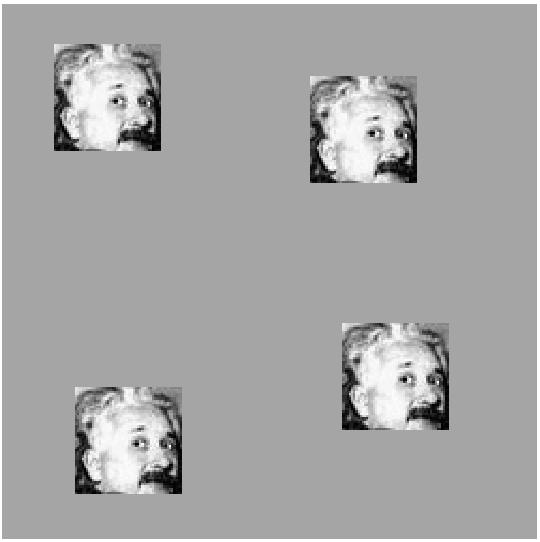
\includegraphics[scale=0.5]{micrograph_Einstein_example_clean}
		\caption{$\sigma = 0$}
	\end{subfigure}%
	\begin{subfigure}[h]{0.33\textwidth}
		\centering
		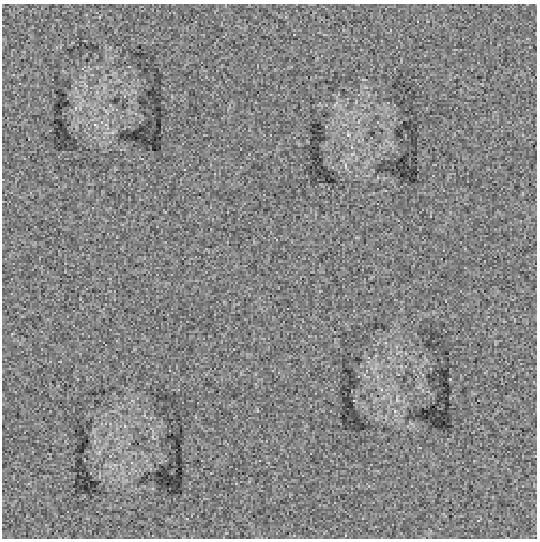
\includegraphics[scale=0.5]{micrograph_Einstein_example_s05}
		\caption{$\sigma = 0.5$}
	\end{subfigure}
	\begin{subfigure}[h]{0.33\textwidth}
		\centering
		
\includegraphics[scale=0.5]{micrograph_Einstein_example_s3}
		\caption{$\sigma = 3$}
	\end{subfigure}
	\caption{\label{fig:micro_example} Example of data sequences (micrographs) of size $250\times 250$ with additive i.i.d./ Gaussian noise with variance $\sigma^2$. Each micrograph contains four occurrences of a $50 \times 50$ image of Einstein.}	
\end{figure}


\paragraph{Autocorrelation analysis.}
In order to recover the signal from the data, we use autocorrelation analysis.
In a nutshell, the method consists of two stages. First, we estimate a mixture (i.e., linear combination) of the low--order autocorrelation functions of the signals from the data. These quantities can be estimated, to any desired accuracy, if individual occurrences are separated by the size of the signal and  each signal appears sufficiently many times in the data. There is no need to detect individual occurrences, knowing the number of signal occurrences $M$ or the noise level.
In the second stage, the signals are estimated from the mixed autocorrelations using a nonconvex least-squares (LS) or phase retrieval algorithms; see Section~\ref{sec:methods}.
This method requires only one pass over the data and can recover the signals in any $\SNR$ level, if the signals appear enough times in the data. As a side note, we mention that expectation-maximization---a popular framework in SPR---is intractable for this problem (see Appendix~\ref{sec:theory}  for more details). 

\section{Results}

%\TODO{Here we should say that we can afford to work only with non-biased terms}

\TODO{Revise to explain $K = 1$ experiment first, then explain $K = 3$.}
\TODO{TB: we should remove the ``long estimation" from the plots}

In this section we show numerical results, while leaving the specific details of the experiments for Section~\ref{sec:methods}. In the first experiment, we estimated Einstein's image from micrographs with $\sigma=3$ . An example for a micrograph appears in the right panel of Figure~\ref{fig:micro_example}. As initial guess, we picked Newton image. If the algorithm was prone to model bias, we would expect to get as an output an image that resembles Newton, similarly to the ``Einstein from noise'' effect. Nonetheless, the more data we collect, the better the reconstruction.\TODO{We have a movie in the supplementary material.}

\begin{figure}[h!]
	\centering
	\begin{subfigure}[h]{0.25\textwidth}
		\centering
		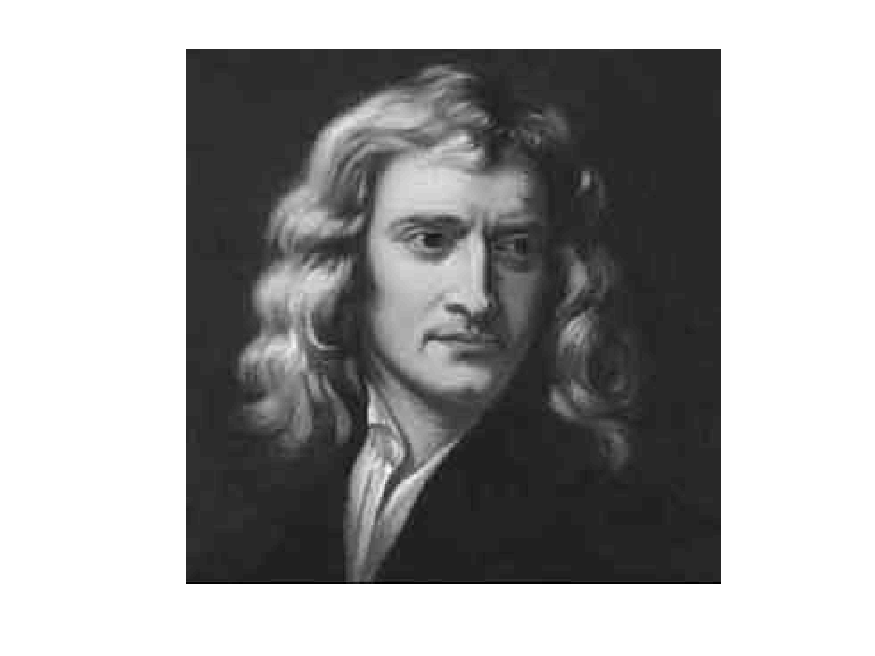
\includegraphics[scale=0.4]{Newton}
		\caption{Newton  (model)}
	\end{subfigure}%
	\begin{subfigure}[h]{0.25\textwidth}
		\centering
		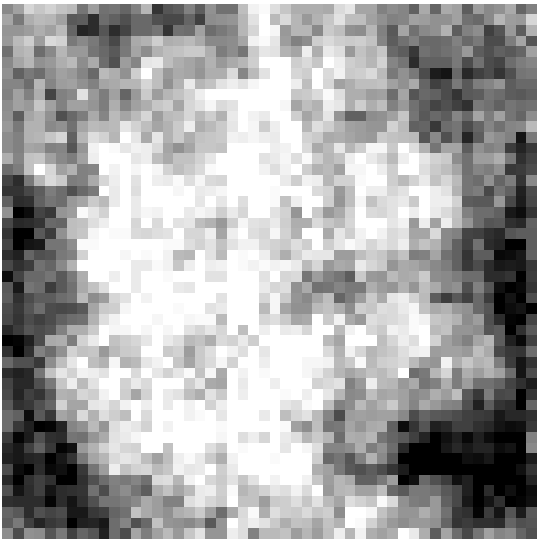
\includegraphics[scale=0.4]{Einstein_100}
		\caption{$P =10^2$}
	\end{subfigure}%
	\begin{subfigure}[h]{0.25\textwidth}
		\centering
		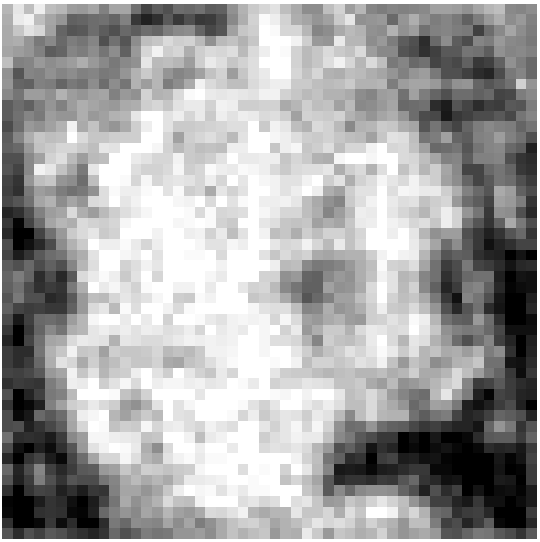
\includegraphics[scale=0.4]{Einstein_1e3}
		\caption{$P =10^3$}
	\end{subfigure}%
	\begin{subfigure}[h]{0.25\textwidth}
		\centering
		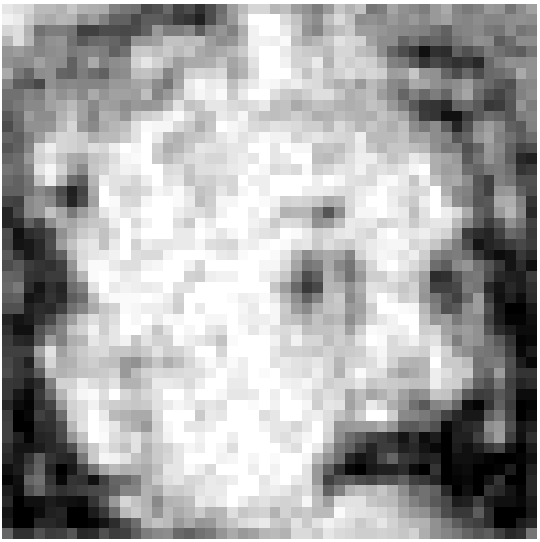
\includegraphics[scale=0.4]{Einstein_1e4}
		\caption{$P = 10^4$}
	\end{subfigure}%
	\caption{\label{fig:Einst_example} Recovery of Einstein image. The algorithm is initialized by the image of Newton. We show estimations of Einstein using $P=10^2,10^3$ and $10^4$ number of micrographs, each contains $860$ image occurrences on average. The normalized recovery error is $0.555$, $0.3988$ and $0.2907$, respectively. The normalized error in recovering the power spectrum was $69.1\times10^{-3} $, $21.7\times10^{-3} $ and $6.8\times10^{-3}$, respectively. \TODO{This image will be more impressive in the future}}	
\end{figure}


Here we should describe the 1-D experiments.


\begin{figure}[t]
	\centering
	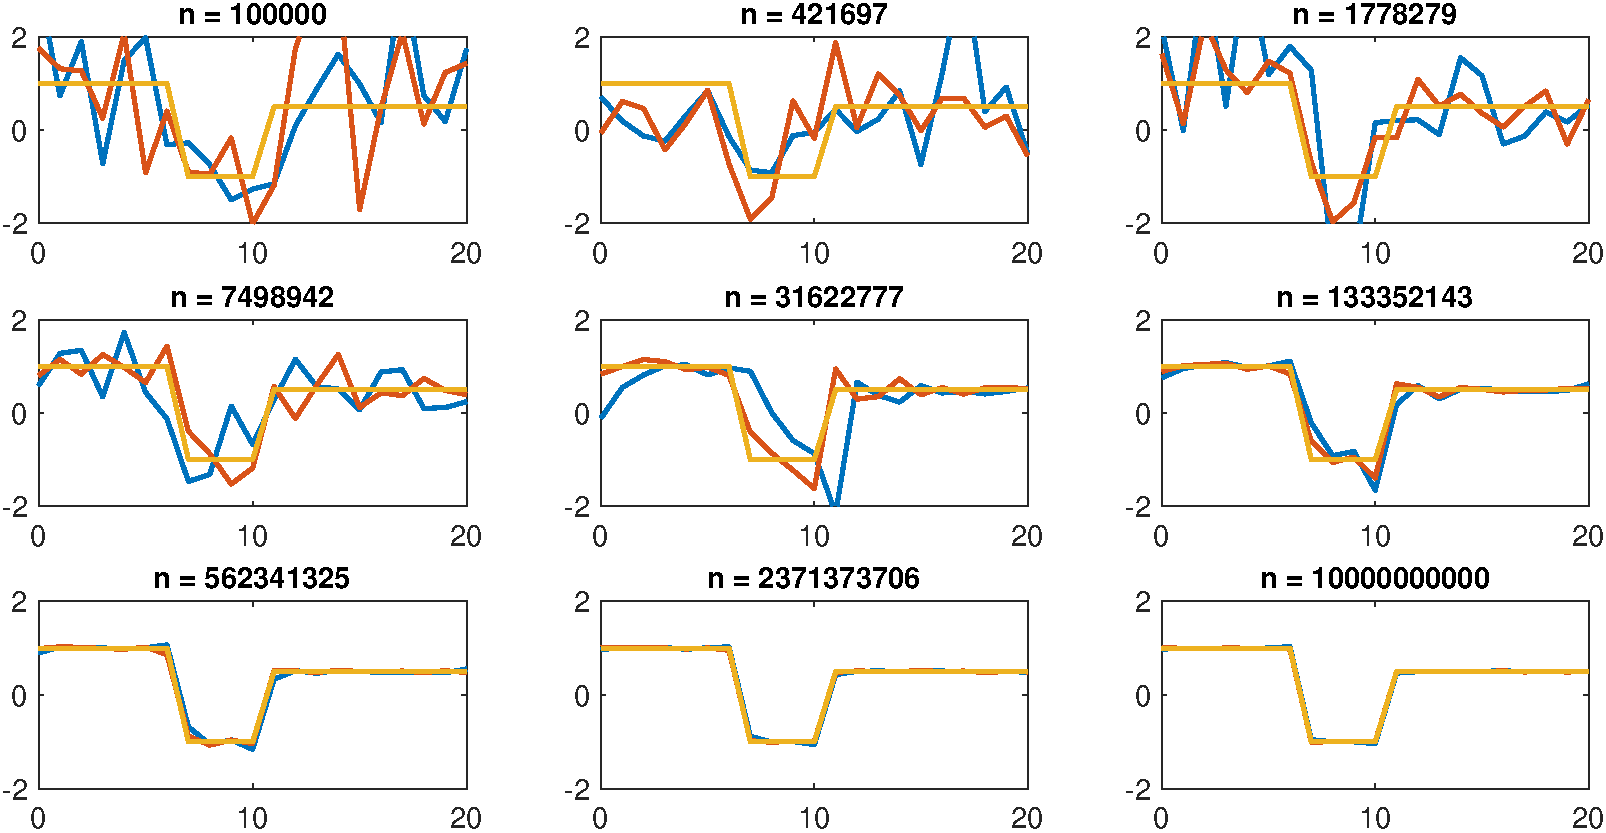
\includegraphics[scale=0.6]{XP_1D_homogeneous_new_ROI/progressive_n10000000000_107521}
	\caption{\TODO{...} \TODO{This figure is with new ROI method based on loss functions}}
	\label{fig:1Dhomosignals}
\end{figure}

\begin{figure}[t]
	\centering
	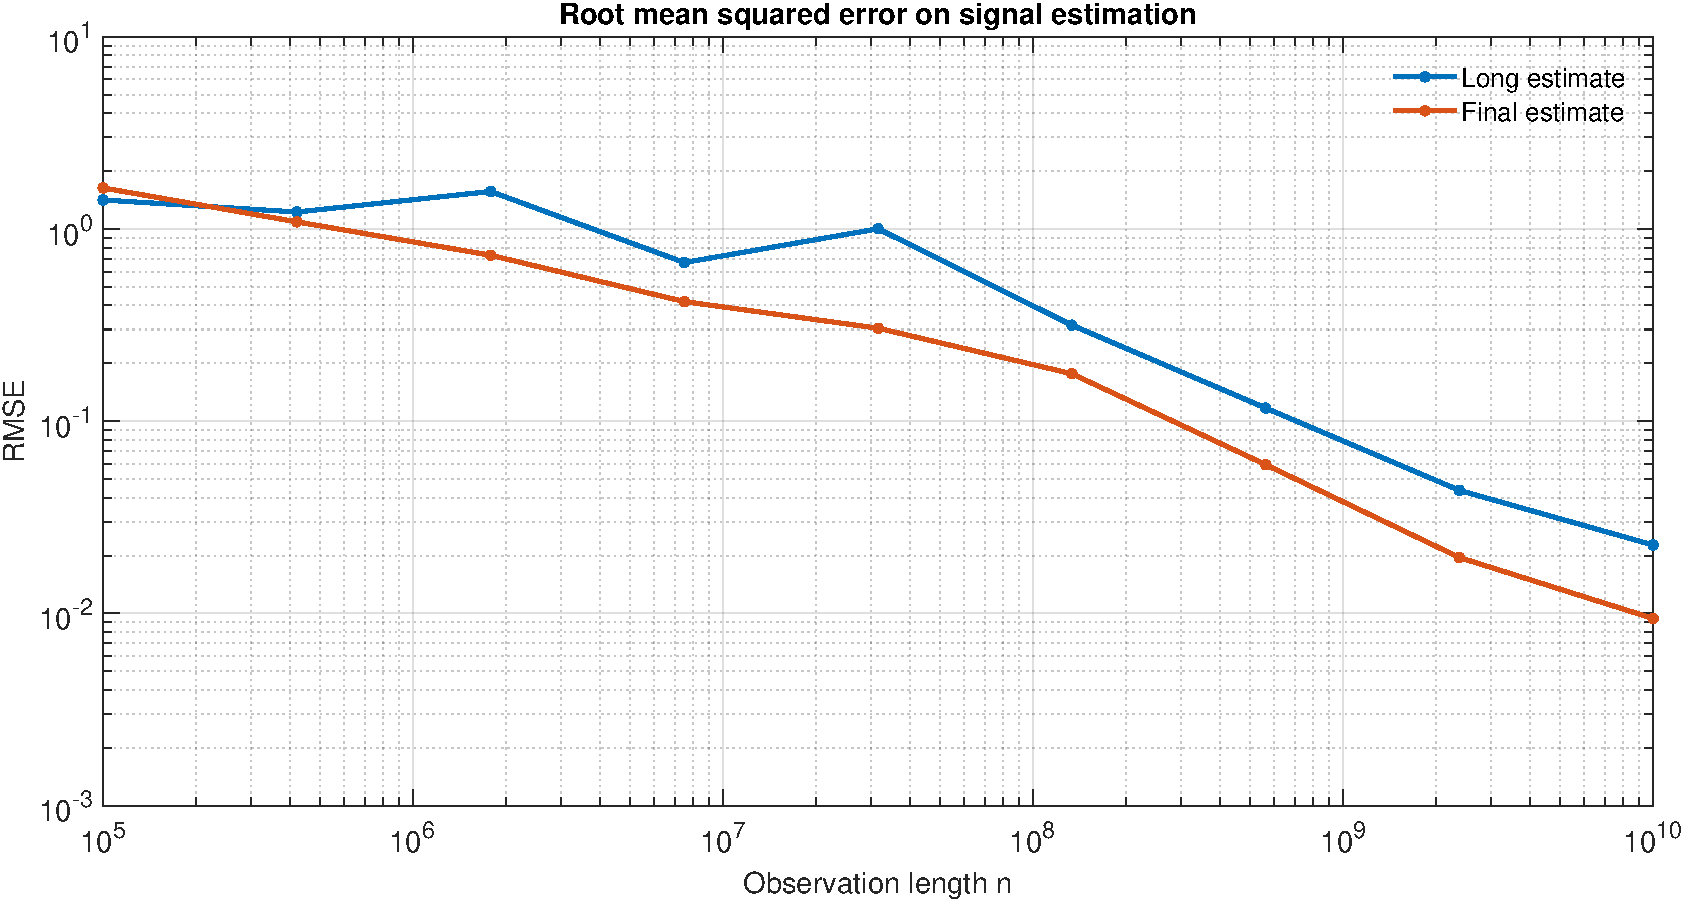
\includegraphics[width=0.7\linewidth]{XP_1D_homogeneous_new_ROI/progressive_RMSE_n10000000000_107521}
	\caption{\TODO{...} \TODO{This figure is with new ROI method based on loss functions}}
	\label{fig:1DhomoRMSE}
\end{figure}

\begin{figure}[t]
	\centering
	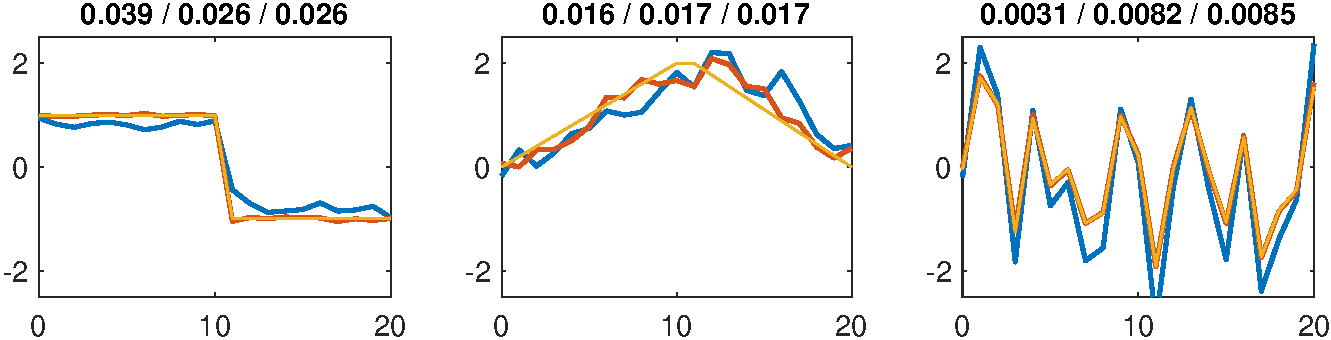
\includegraphics[width=0.9\linewidth]{XP_1D_heterogeneous/data_example_heterogeneous_n_24600000000_604392_fig1}
	\caption{\TODO{Thin yellow is ground truth; blue is ROI of first optimization; red is final estimation. Relative error for blue is .37, and .13 for red. Individual relative errors of the red estimates: 0.0239393 / 0.208925 / 0.0335956}}
	\label{fig:1Dheterosignals}
\end{figure}



\section{Discussion}

All current SPR algorithms start with a particle picking stage which is prone to model bias. 
In this paper, we propose to examine the possibility to bypass particle picking and estimate the particle directly from the micrograph. To this end, we examine a simplified model that share some similarities with the SPR problem. The proposed reconstruction method is based on autocorrelation analysis, 
somewhat similar to a technique proposed by Kam which can be used for ab inito modeling~\cite{kam1980reconstruction,levin20173d,singer2018mathematics}. 
That being said, the SPR model is far more complicated thans the model presented here. In a future research, we hope to bridge this gap.

Our results rely on two core assumptions that are not necessarily met by in an SPR experiment.  
First, we modeled the background information as i.i.d.\ additive noise. In practice, the background information may be structured or depend on the signal. However, methods based on autocorrelation estimation are quite flexible and in many cases can tolerate mismatch of the noise statistical model.

In addition, we assumed that the signal occurrences are all separated, see~\eqref{eq:spacing}. 
This separation can be induced by careful experiment design \TODO{???}. 
If the signals are not separated, one can introduce a new variable that represents the distribution of the spacing between signal occurrences and then compute explicitly the relation between the autocorrelation of the data and the signals. It is yet to be studied under what conditions on this distribution one can estimate the signals. 

%The first entry $p[1]$ will represent the probability that two consecutive signals are separated by only one entry, $p[2]$ the probability for spacing of two entries and so on. Using this auxiliary variable $p$, one can write explicitly the relation between the autocorrelation functions of the data and those of the signal in a similar way to~\eqref{eq:data_ac}. 
%An interesting question is  under what conditions on $p$ and the signals, one can estimate the signals from the data.


\section{Methods} \label{sec:methods}


\paragraph{Mathematical model}

Let $x_1,\ldots,x_K\in\RL$ be the sought signals and let $y\in\RN$ be the data. 
The forward model can be posed as a mixture of \emph{blind deconvolution} problems between binary signals and the target signals $x_i$:
\begin{equation} \label{eq:model}
y = \sum_{i=1}^K x_i\ast s_i + \varepsilon,\quad \varepsilon\sim\mathcal{N}(0,\sigma^2 I).
\end{equation}
%We model the background information as i.i.d.\ Gaussian noise with zero mean and $\sigma^2$ variance. 
The nonzero values of each  $s_i\in\{0,1\}^N$ determine the position of the occurrences of the corresponding $x_i$. 
We denote the set of these nonzero values by 
 $\mathcal{S}_i$ and its cardinality by $\vert \mathcal{S}_i\vert = M_i$. 
By assuming that all $\mathcal{S}_i$'s are disjoint,  we let $s = \sum_{i=1}^Ks_i$, $\mathcal{S} = \bigcup_{i=1}^{K} \mathcal{S}_i$ and  $\vert \mathcal{S}\vert :=M =  \sum_{i=1}^{K}M_i$.  Neither the $M_i$'s nor $M$ are assumed to be known. Literature survey on blind deconvolution and related problems is given in Appendix~\ref{sec:related_literature}.

In order to estimate the mixture of autocorrelations, we assume that the support of $s$ is not clustered. In particular,
\begin{equation} \label{eq:spacing}
\text{For all }  i,j\in\mathcal{S}, \, i\neq j,  \quad  \vert i-j \vert\geq L-1.  
\end{equation}
The goal of the problem is to estimate $x_1,\ldots,x_K$ from $y$.


%
%\section{Autocorrelation analysis}   \label{sec:autocorrelation}
%
%Our method for estimating the signals is composed of two stages. 
%First, we use the autocorrelation functions of the data to estimate a mixture (i.e., linear combination) of the $K$ signal's autocorrelations. The mixed autocorrelation can be estimated to any accuracy, in any $\SNR$ level, if $M$ is large enough and the spacing condition~\eqref{eq:spacing} is met. Then, we  use a nonconvex LS  to estimate the signals from their mixed autocorrelations. 
%In this section, we elaborate on the autocorrelation functions and their estimations, while the precise recovery procedure, based on nonconvex optimization, will be discussed in detail in the next section.

\paragraph{Aperiodic autocorrelation functions}
%\subsection{Aperiodic autocorrelation functions} \label{sec:aperiodic_ac}

For the purpose of this paper, we need the first three (aperiodic) autocorrelation functions. The first-order autocorelation is the mean of the signals. For  
$z\in\RL$ and $k\geq 2$, the autocorrelation of order $k$ is defined for any integer shifts $\ell_1, \ldots, \ell_{k-1}$ by
\begin{align}
	a_z^k[\ell_1,\ldots,\ell_{k-1}]  & = \sum_{i=-\infty}^{+\infty} z[i]z[i+\ell_1]\ldots z[i+\ell_{k-1}],
	\label{eq:ac_general}
\end{align}
where indexing of $z$ out of the bounds $0, \ldots, L-1$ is zero-padded, as usual.
Explicitly, the first three autocorrelations are
\begin{align} 
	a_z^1 & = \sum_{i=0}^{L-1} z[i], \nonumber\\
	a_z^2[\ell] & = \sum_{i = \max\{0, -\ell\}}^{L-1 + \min\{0, -\ell\}} z[i]z[i+\ell], \nonumber\\
	a_z^3[\ell_1,\ell_2] & = \sum_{i = \max\{0, -\ell_1, -\ell_2\}}^{L-1 + \min\{0, -\ell_1, -\ell_2\}} z[i]z[i+\ell_1]z[i+\ell_2]. \label{eq:ac_special}
\end{align}
Note that the autocorrelation functions are symmetric so that $a_z^2[\ell] = a_z^2[-\ell]$ and $$a_z^3[\ell_1,\ell_2] = a_z^3[\ell_2,\ell_1]=a_z^3[-\ell_1,\ell_2-\ell_1].$$
%Additionally, if the moments of the signal depend only on the difference between the indices (Toeplitz structure), then they are equivalent to the autocorrelation functions.

\paragraph{Estimating the autocorrelation function of a single signal}

We first consider the problem of estimating the autocorrelations of a single signal from the data. 
The main principles carry through for $K>1$ as will be shown next.  

%In order to estimate the autocorrelations of the signal, we first compute the first $L$ entries of the data's autocorrelations. 
For the purpose of the analysis, we consider  the asymptotic regime where $M,N\to\infty$, while preserving fixed ratio. 
Specifically, we define the ratio of the measurement occupied by  the signal as
\begin{equation}
\gamma = \frac{M L}{N}.
\end{equation}
Under the spacing constraint~\eqref{eq:spacing}, we have $\gamma\leq\frac{L}{2L-1}\approx 1/2$.

The main pillar of this work is the following simple observation.
If the support signal $s$ satisfies the spacing constraint~\eqref{eq:spacing}, then the first $L$ entries of the data autocorrelations converge 
to a scaled, biased, version of the signal's autocorrelation:
\begin{align}
\lim_{N\to\infty} a_y^1 & = \gamma a_{x}^1, \nonumber\\
\lim_{N\to\infty} a_y^2[\ell] & = \gamma a_{x}^2[\ell] +\sigma^2\delta[\ell], \label{eq:data_ac_k1} \\
\lim_{N\to\infty} a_y^3[\ell_1,\ell_2] & = \gamma a_{x}^3[\ell_1,\ell_2] + \sigma^2\gamma a_{x}^1 \big(\delta[\ell_1,0]+\delta[0,\ell_2]+\delta[\ell_1,\ell_2]\big), \nonumber
\end{align}
for $\ell,\ell_1,\ell_2=0,\ldots L-1$, and where $\delta$ denotes the Kronecker delta function. 
%These relations are proven in Appendix~\ref{sec:autocorrelation_computation}.

\paragraph{Estimating the autocorrelation function of a multiple signals}

As before, we consider  the asymptomatic regime where $M_1,\ldots,M_K,N\to\infty$, while preserving fixed ratios
\begin{align}
	\gamma_k = \frac{M_k L}{N}, \quad \gamma = \sum_{k=1}^K\gamma_k.
\end{align}
If the support $s$ satisfies the spacing constraint~\eqref{eq:spacing}, then one can estimate the mixture of the $K$ signals'  autocorrelations, similarly to~\eqref{eq:data_ac_k1}: 
\begin{align}
\lim_{N\to\infty} a_y^1 & = \sum_{k=1}^K\gamma_k a_{x_k}^1, \nonumber\\
\lim_{N\to\infty} a_y^2[\ell] & = \sum_{k=1}^K\gamma_k a_{x_k}^2[\ell] +\sigma^2\delta[\ell],  \label{eq:data_ac}\\
\lim_{N\to\infty} a_y^3[\ell_1,\ell_2] & = \sum_{k=1}^K\gamma_k a_{x_k}^3[\ell_1,\ell_2] + \sigma^2\left(\sum_{k=1}^K\gamma_k a_{x_k}^1\right)(\delta[\ell_1,0]+\delta[0,\ell_2]+\delta[\ell_1,\ell_2]), \nonumber
\end{align}
This relation is proven in  Appendix~\ref{sec:autocorrelation_computation}.

\paragraph{Numerical experiments details}

\TODO{We may want to split it into two sections. Here we could give a short description with the LS estimator and the RRR. In the supplementary material we can provide all other details. }

For the 1D experiment, we fix $K = 3$ signals of length $L = 21$, as depicted in Figure~\TODO{ref}. Following the data model described in Section~\TODO{ref}, we generate an observation $y$ of length $24.6 \cdot 10^9$. Each of the three signals appears, respectively (and approximately) $300 \cdot 10^6$, $200 \cdot 10^6$ and $100 \cdot 10^6$ times in $y$, such that at least $L-1$ zeros separate two occurrences of any signals. This is done by randomly selecting $600 \cdot 10^6$ placements in $y$, one at a time with an accept/reject rule based on the separation constraint and locations picked so far. For each placement, one of the three signals is picked at random proportionally to the desired number of occurrences of each. Then, i.i.d.\ Gaussian noise with mean zero and standard deviation $\sigma = 3$ is added, to form the observed $y$. The SNR of $y$
% sqrt((m_want*sum(X.^2)')/(sigma^2*n))
is about 1/12.
%Given the scaling of the target signals (whose median absolute value for the entries is at or below one),
This is enough noise to make cross-correlations of $y$ even with the true signals display peaks at random locations, uninformative of the actual locations of the signal occurrences. Thus, we contend that it would be difficult for any algorithm to locate the signal occurrences, let alone to classify them according to which signal appears where.

\TODO{TB: I would place the equation counting argument in the theory section in the paragraph of open questions (I marked th place)}
Given the observation $y$, we proceed to compute the moments. The first-order moment is straightforward. For second-order moments, notice from equation~\eqref{eq:data_ac} that $a_y^2[\ell]$ suffers no bias for $\ell$ in $1$ to $L-1$. Thus, we omit $\ell = 0$, which has the practical effect that we need not know $\sigma$ to estimate the moments. Likewise, for third-order moments, $a_y^3[\ell_1, \ell_2]$ for $0 \leq \ell_1, \ell_2 \leq L-1$ such that $\ell_2 \leq \ell_1$ includes all relevant moments for our purpose \TODO{Do we want to include a figure to explain why that is?}, and we further exclude any such that $\ell_1, \ell_2$ or $\ell_1 - \ell_2$ are zero to avoid biased elements---there are $\frac{(L-1)(L-2)}{2}$ remaining moments. As a result, it is unnecessary to estimate $\sigma$. We have \TODO{TB: We may want to put this calculation is the last paragraph of Section 3.1 }
\begin{align*}
1 + (L-1) + \frac{(L-1)(L-2)}{2} = \frac{1}{2} L (L-1) + 1
\end{align*}
moments in total. In practice, these are computed on disjoint segments of $y$ of length $100\cdot10^6$ and added up, without correction for the junction points. Segments are handled sequentially on a GPU, as GPUs are particularly well suited to execute simple instructions across large vectors of data. If multiple GPUs are available, segments can of course be handled in parallel.

Having computed the moments of interest, we now estimate signals $x_1, \ldots, x_K$ and coefficients $\gamma_1, \ldots, \gamma_K$ which agree with the data. We choose to do so by running an optimization algorithm on the following nonlinear least-squares problem:
\begin{multline}
\min_{\substack{\hat x_1, \ldots, \hat x_K \in \reals^{W} \\ \hat \gamma_1, \ldots, \hat \gamma_K > 0}} w_1 \left( a_y^1 - \sum_{k=1}^K \hat \gamma_k a_{\hat x_k}^1 \right)^2 + w_2 \sum_{\ell = 1}^{L-1} \left( a_y^2[\ell] - \sum_{k=1}^K \hat \gamma_k a_{\hat x_k}^2[\ell] \right)^2 + \\ w_3 \sum_{\substack{2\leq\ell_1\leq L-1 \\ 1 \leq \ell_2 \leq \ell_1-1}} \left( a_y^3[\ell_1, \ell_2] - \sum_{k=1}^K \hat \gamma_k a_{\hat x_k}^3[\ell_1,\ell_2] \right)^2.
\label{eq:optim1D}
\end{multline}
where $W \geq L$ is the length of the sought signals and \TODO{explain $w_i$'s: currently they are $w_1 = 1/2, w_2 = 1/2n_2, w_3 = 1/2n_3$, where $n_2, n_3$ are the number of moments used: $n_2 = L-1$, $n_3 = \frac{(L-1)(L-2)}{2}$. Issue is: this is not very smart..}. Setting $W = L$ (as is a priori desired) is problematic because the above optimization problems appears to have numerous poor local optimizers.
%Since we can only initialize randomly at first, this approach would often fail in practice. Alternatively,
Thus, we first run the optimization with $W = 2L-1$. This problem appears to have fewer poor local optima, perhaps because the additional degrees of freedom allow for more escape directions. Since we hope the signals estimated this way correspond to the true signals zero-padded to length $W$, we extract from each one a subsignal of length $L$ (with cyclic indexing \TODO{we should understand / explain this}) that has largest $\ell_2$-norm. This estimator is then used as initial iterate for~\eqref{eq:optim1D}, this time with $W = L$. We find that this procedure is reliable for a wide range of experimental parameters. To solve~\eqref{eq:optim1D}, we run the trust-region method implemented in Manopt~\cite{manopt}, which allows to treat the positivity constraints \TODO{I might need a reference for this} on coefficients $\hat \gamma_k$. Notice that the cost function is a polynomial in the variables, so that it is straightforward to compute it and its derivatives.
\TODO{Should we do variable projection for the gammas, that is, exploit the fact the problem is a regular least squares in the gammas (up to the positivity constraints) to substitute the explicit optimum for them? Not sure it's worth the effort. -- Ok, it's probably not a good idea, because even with fixed gammas to the correct value, optimization takes a while.}
\TODO{Do we still need to stress at this point that the optimization part has complexity independent of length of observation? Should be pretty clear at this point already.}





\bibliographystyle{plain}
\bibliography{ref}



\appendix

\section{Autocorrelation estimations} \label{sec:autocorrelation_computation}

Throughout the proof, we consider the case of one signal $K=1$. The extension to $K>1$ is straightforward by averaging the contributions of all signal with  appropriates weights, see~\cite{boumal2017heterogeneous}. 

Let us define
\begin{equation}
\gamma = \lim_{N\to\infty} \frac{M_NL}{N}<1.
\end{equation}
With a bit abuse of notation, $M_N$ stresses that $M$ is a function of $N$. Indeed, by assuming $M_N=\Omega(N)$, we deduce $\gamma>0$.
We start by considering the first autocorrelation of the data
\begin{equation}
a_y^1 = \sum_{i=0}^{N-1} y[i] = \frac{1}{N/L}\sum_{j=0}^{M_N-1}\frac{1}{L}\sum_{i=0}^{L-1}x[i] + \underbrace{\frac{1}{N}\sum_{i=0}^{N-1}\varepsilon[i]}_{\text{noise term}} \xrightarrow{a.s.}\gamma a_x^1,
\end{equation}
where the noise term converges to zero almost surely (a.s.) by the law of large numbers.

We proceed with the second autocorrelation for fixed $\ell\in[0,\ldots,L-1]$. We can compute:
\begin{equation}
\begin{split}
a_y^2[\ell] & = \frac{1}{N}\sum_{i=0}^{N-1-\ell}y[i]y[i+\ell] \\
& \underbrace{\frac{1}{N}\sum_{j=1}^{M_N}\sum_{i=0}^{L-\ell-1}x[i]x[i+\ell]}_{\text{signal term}} + \underbrace{\frac{1}{N}\sum_{i=0}^{N-1-\ell}\varepsilon[i]\varepsilon[i+\ell]}_{\text{noise term}},
\end{split}
\end{equation}
where the cross terms between the signal and the noise vanish  almost surely in the limit $N\to\infty$. 

We treat the signal and noise terms separately. We first break the signal term into $M_N$ different sums, each contains one copy of the signal, and get
\begin{equation} \label{eq:2nd_moment_signal_term}
\frac{1}{N}\sum_{j=1}^{M_N}\sum_{i=0}^{L-\ell-1}x[i]x[i+\ell] = \frac{M_NL}{N}\frac{1}{L}\sum_{i=0}^{L-\ell-1}x[i]x[i+\ell] = \gamma a_x^2[\ell].
\end{equation}
Similarly, for $\ell\neq 0$, we can break the noise term into a sum of independent terms 
\begin{equation}
\frac{1}{N}\sum_{i=0}^{N-1-\ell} \varepsilon[i]\varepsilon[i+\ell] = \frac{1}{\ell}\sum_{i=0}^{\ell-1}\frac{1}{N/\ell}\sum_{j=0}^{N/\ell -1} \varepsilon[j\ell + i] \varepsilon[(j+1)\ell + i].
\end{equation}
Each term of $\frac{1}{N/\ell}\sum_{j=0}^{N/\ell -1} \varepsilon[j\ell + i] \varepsilon[(j+1)\ell + i]$ is an average of $N/\ell$ independent terms with expectation zero, and thus converges to zero almost surely as $N\to\infty$.
If $\ell=0$, 
\begin{equation}
\frac{1}{N}\sum_{i=0}^{N-1} \varepsilon^2[i] \xrightarrow{a.s.} \sigma^2.
\end{equation}

We are now moving to analyze the third-order autocorrelation. Let us fix $\ell_1\geq\ell_2$ and recall that 
\begin{equation*}
a_y^3[\ell_1,\ell_2] = \sum_{i=0}^{N-1-\ell_1} y[i]y[i+\ell_1]y[i+\ell_2]. 
\end{equation*}
Writing explicitly in terms of signal and noise, the sum can be broken into eight terms. The first contains only signal terms (does not see noise) and converges to $\gamma a_x^3$ from the same reasons as~\eqref{eq:2nd_moment_signal_term}. Three other terms contain the product of two signal entries and one noise term. Since the noise is independent of the signal and has zero mean, these terms go to zero almost surely.

We next analyze the contribution of the term composed of triple products of noise terms. For $\ell_1\neq 0$, this sum can be formulate as follows:
\begin{equation*}
\sum_{i=0}^{N-1-\ell_1} \varepsilon[i]\varepsilon[i+\ell_1]\varepsilon[i+\ell_2] = \frac{1}{\ell_1}\sum_{i=0}^{\ell_1-1}\frac{1}{N/\ell_1}\sum_{j=0}^{N/\ell_1 -1 }\varepsilon[j\ell_1+i]\varepsilon[(j+1)\ell_1+i]\varepsilon[j\ell_1+i+\ell_2].
\end{equation*}
For each fixed $i$, we sum of over $N/\ell_1$ independent variables that goes to zero almost surely. For $\ell_1=\ell_2=0$, we get a some of $N$ independent variables, each one is a triple product of Gaussian variables with zero mean and therefore has zero expectation. 

To complete the analysis, we consider the three terms composed of the product of two noise terms and one signal entry. Most of these terms converge to zero almost surely because of independency between the noise entries. For $\ell_1=0, \ell_2=0$ and $\ell_1=\ell_2$,  a simple computation shows that the sum converges to $\gamma\sigma^2a_x^1$; c.f.~\cite{boumal2017heterogeneous}.


\section{Related literature} \label{sec:related_literature}

\paragraph{Blind deconvolution.}
Blind deconvolution is a longstanding problem, arising in a variety of engineering and scientific applications, such as astronomy, communication, image deblurring, system identification and optics; see~\cite{jefferies1993restoration,shalvi1990new,ayers1988iterative,abed1997blind}, just to name a few. 
To make the problem well-posed, we must  assume some prior knowledge or  structure. 
In our case, the prior information is that $s$ is a binary signal that satisfies the separation constraint~\eqref{eq:spacing}. 
Other settings of blind deconvolution problems have been analyzed recently, see for instance~\cite{ahmed2014blind,li2016identifiability,li2016rapid,ling2015self,ling2017blind,chi2016guaranteed}
where the focus is on high $\SNR$ regimes.


An important feature of the problem under consideration is that while both $x_i$'s and $s_i$'s are unknown, the goal is merely to estimate the $x_i$'s. The  $s_i$'s  are referred to as \emph{nuisance  variables}. Indeed, in many blind deconvolution applications the sole purpose is to recover one of the unknown signals. For instance, in image deblurring, both the blurring
kernel and the high-resolution image are unknown, but the primary goal is only
to sharpen the image.

\paragraph{The impossibility of detection in low $\SNR$.}
If $x$ is known and $K=1$, then a sparse signal can be estimated by linear programming  in the high $\SNR$ regime, e.g.,~\cite{azais2015spike,denoyelle2017support,bendory2016robust,bendory2017robust,bernstein2017deconvolution}. However, in the low $\SNR$ regime, estimating the binary sparse signal $s$ is impossible. To see that, suppose that an oracle provides us $M$ windows of length $W>L$, each contains one copy of $x$. That is to say, we get a series of windows of length $W$, each one contains a signal at an unknown location. 
Estimating the position of the known signal within each  window is an easier problem than detecting the support of $s$. 
Nevertheless, even this problem is impossible in the low $\SNR$ regime~\cite{aguerrebere2016fundamental}. Therefore, we conclude that detecting the nonzero values of $s$ is impossible in low $\SNR$. As aforementioned, this work focuses on this regime and examines under what conditions we can estimate the signals, despite the impossibility of detecting their individual occurrences.

\paragraph{System identification.}
For $K=1$, our problem can be also interpreted as a special case of the system identification problem. Similarly to~\eqref{eq:model}, the system identification forward model takes the form
\begin{eqnarray}
y = x\ast w + \varepsilon,  
\end{eqnarray} 
where $x$ is the unknown signal (``system''), $w$ is an unknown, random, input sequence and $\varepsilon$ is an additive noise.   
%The problem has also been studied in the case of a known input $w$~\cite{pillonetto2010new,dinuzzo2015kernels,bottegal2016robust}. 
The goal of this problem is to estimate $x$, usually referred to as ``identifying the system.'' The question of identifiability of $x$ under
this observation model is addressed for certain Gaussian and non-Gaussian $w$ in~\cite{benveniste1980robust,kormylo1983identifiability}.
In the special case where $w\in\{0,1\}^N$, satisfying the spacing requirement~\eqref{eq:spacing}, we obtain our
model in the  case of a single signal ($K = 1$).

Likelihood-based methods seek to maximize the likelihood function for $x$,
given the observed signal $y$. Solving this optimization exactly is typically
intractable, and thus heuristic methods are used instead. One proposed technique is to use Markov Chain Monte Carlo (MCMC); in special
cases, including the case where $w$ is binary, EM has been used~\cite{cappe1999simulation}.
The EM method is based upon a certain ``forward-backward'' procedure
used in hidden Markov models~\cite{rabiner1989tutorial}. 
However, the complexity of this procedure is still nonlinear in $N$, and therefore its usage is limited for big data sets.   
Another paper considers parameterized models for multiple distinct signals, as in our heterogeneity framework ($K>1$)~\cite{andrieu2001bayesian}.
Their proposed solution is an MCMC algorithm tailored for their specific parametrized problem.

Because likelihood methods are computationally expensive, methods based
on recovery from moments, which are akin to our method, have
also been previously used for system identification. 
Methods based on the third- and fourth-order moments are described and analyzed in~\cite{lii1982deconvolution,giannakis1989identification,tugnait1984identification}.

\section{Theory} \label{sec:theory}

A one-dimensional signal is determined uniquely and stably by its third-order autocorrelation as proven in the following simple proposition.
\begin{proposition} \label{prop:uniqueness}
	Let $z\in\RL$ and suppose that $z[0]$ and $z[L-1]$ are nonzero. Then:
	\begin{itemize}
		\item \textbf{Uniqueness:} 	 $z$  is determined uniquely from  $a_z^2$ and $a_z^3$.
		\item \textbf{Finite sensitivity:} 	Suppose we can only measure $\tilde{a_z^3}[k,L-1] = a_z^3[k,L-1]+\upsilon$ and that $\vert z[0]z[L-1]\vert \geq \delta>0$.
		Then,  $\hat{z}[k] =\frac{\tilde{a_z^3}[k,L-1]}{a_z^2[L-1]} $ satisfies $\vert \hat{z}[k] - z[k]\vert\leq \frac{\vert \upsilon\vert }{\delta}$. 
	\end{itemize}
	\begin{proof}
		By assumption $a_z^2[L-1] = z[0]z[L-1]\neq 0$.
		Then, the uniqueness results, for all $k=0,\ldots L-1$,  follows from:
		\begin{equation*}
		a_z^3[k,L-1] = z[0]z[k]z[L-1].
		\end{equation*}
		In addition, 
		\begin{equation*}
		\hat{z}[k] = \frac{\tilde{a_z^3}[k,L-1]}{a_z^2[L-1]} = z[k]+\frac{\upsilon}{a_z^2[L-1]} \quad \Rightarrow \quad \vert \hat{z}[k] - {z}[k]\vert \leq \frac{\vert\upsilon\vert}{\delta}.
		\end{equation*} 
	\end{proof}
\end{proposition}

A few remarks are in order. 
First, the second result of Proposition~\ref{prop:uniqueness} shows that there exists a very simple estimator that has finite sensitivity. In the next numerical experiments we use an estimator based on nonconvex LS that shows empirical robustness to additive noise, in accordance with related problems~\cite{bendory2017bispectrum,boumal2017heterogeneous}. 
Second, these results carry through to signals of any dimension.
Third, if the spacing condition~\eqref{eq:spacing} holds, then the length of the signal can be determined from the autocorrelations and 
therefore the assumption that the first and last entries are nonzero is met. In particular, if~\eqref{eq:spacing} holds for some spacing $W\geq L$, then $a_z^2[i]=0$ for all $i>L-1$.
Finally, computing the $d$th autocorrelation amplifies the variance of the noise by a factor $d$ in the low $\SNR$ regime. Therefore, if we can estimate $a_z^3$ up to small perturbation, it implies that we can estimate $a_z^2$ accurately as the proposition assumes. 

Considering the third-order autocorrelation is also a necessary condition to determine a signal from its autocorrelations. Indeed, the second-order autocorrelation of a one-dimensional signal does not determine a signals uniquely~\cite{beinert2015ambiguities,bendory2017fourier}. On the other hand, for dimensions greater than one, almost all signals are determined uniquely, up to sign (phase for the complex signals) and reflection through the origin (with conjugation in the complex case)~\cite{hayes1982reconstruction,hayes1982reducible}. The sign ambiguity can be resolved by the mean of the signal if it is not zero. However,  in order to determine the reflection symmetry, one needs to use additional information.


If the noise level $\sigma^2$ is known, one can estimate the ratio $M/N$ from the first two moments.
\begin{proposition} \label{prop:gamma}
	Let $K=1$, $N\to\infty$ and $\sigma$ fixed. If the mean of $x$ is nonzero, then 
	\begin{equation*}
	\frac{M}{N} = \frac{1}{L}\frac{(a^1_y)^2}{\sum_{j=0}^{L-1}a_y^2[j]-\sigma^2}.
	\end{equation*}
	\begin{proof}
		The proof follows from plugging the explicit expressions of~\eqref{eq:data_ac_k1} into the right hand side of the equality.
	\end{proof}
\end{proposition}

If we use third-order autocorrelation information, then it is possible to estimate both the ratio $M/N$ and $\sigma$ simultaneously.
\begin{proposition} \label{prop:gamma_sigma}
	Let $K=1$, $N\to\infty$ and $\sigma$ fixed. Then, $a_y^1,a_y^2$ and  $a_y^3$ determine the ratio $M/N$ and $\sigma$ uniquely for a generic signal $x$. If $\frac{M}{N}\geq\frac{1}{4(L-1)}$, then it holds for any signal with nonzero mean. 
	\begin{proof}
		See Appendix~\ref{sec:proof_prop_gamma_sigma}.
	\end{proof}
\end{proposition}

From Propositions~\ref{prop:uniqueness} and~\ref{prop:gamma_sigma} we can directly deduce the following:
\begin{corollary}
	Let $K=1$, $N\to\infty$ and $\sigma$ is fixed. Then, the signal, the ratio $M/N$ and $\sigma$ can be recovered from the first three autocorrelation functions if:
	\begin{itemize}
		\item $x$ is generic;
		\item  $x[0],x[L-1]\neq 0$, $x$ has nonzero mean and $\frac{M}{N}\geq\frac{1}{4(L-1)}$.
	\end{itemize}
\end{corollary}

\paragraph{Expectation-maximization.}
Interestingly, expectation-maximization (EM)---a popular algorithm for similar estimation problems, such as Gaussian mixture models and multireference alignment---is intractable for this problem. This is true even if  $K=1$ and the number of signal occurrences $M$ is known.
In particular, in each iteration, EM assigns a probability to any feasible combination of positioning the current signal estimate in $M$ locations on the grid $\{1,\ldots,N\}$.
In total, even when excluding forbidden combinations due to the spacing constraint, there are $O(N^M)$ such combinations.


\paragraph{Open theoretical questions.}


The minimal order of data statistics used to get an accurate estimation of a signal is important to understand, in the asymptotic $\SNR$ regime, the sample complexity of the problem.
In methods which are based on detection and averaging, the number of signals occurrences  must scale like $1/\SNR$. On the contrary, the required number signal occurrences using the autocorrelation analysis should scale like $1/\SNR^d$  to retain a constant estimation error. Accordingly, in our  method, $M$ must scale like $1/\SNR^3$. We believe that similarly to the closely-related problem of multirefrence alignment~\cite{perry2017sample,abbe2017multireference}, this estimation rate is optimal in the low $\SNR$ regime.

In addition, the  third-order autocorrelation succeeds, empirically, to demix  $K>1$ signals, even without prior knowledge of the $M_i$'s and $\sigma$. Based on the following equation counting, we believe that one can demix up $\approx L/2$ signals. 
\TODO{Here we can add the equations counting argument. Do we want to consider also conjecture on the computational limit?}



\section{Proof of Proposition~\ref{prop:gamma_sigma}} \label{sec:proof_prop_gamma_sigma}

We aim to prove that one can estimate both $\sigma$ and $\beta = M/N$ from the observed first three moments.
To this end, we construct two quadratic equations of $\beta$ from the observed (measured) quantities, independent of $\sigma$.
Then, we show that these equations are independent and therefore $\beta$ is uniquely defined. 
Given $\beta$, we can estimate $\sigma$ using Proposition~\ref{prop:gamma}.
Throughout the proof, it is important to distinguish between observed and unobserved values. 
to this end, we denote the observed values by $E_i$ or $a_y^1,a_y^2,a_y^3$, while using $F_i$ for functions of the signal's autocorrelations. 


Recall that $a_y^1 = \beta(\one^Tx)$ and  
and $a_y^2[0] = \beta\|x\|^2+\sigma^2$, where $\one\in\RL$ stands for vector of ones. Taking the product:
\begin{equation}\label{eq:E1}
\begin{split}
E_1 &:= a_y^1a_y^2[0] =  (\beta(\one^Tx))(\beta\|x\|^2+\sigma^2) \\
& = \sigma^2a_y^1 + \beta^2F_1,
 \end{split}
\end{equation}
where $F_1 := a_x^3[0,0] + \sum_{j=1}^{L-1}(a_x^3[j,j] + a_x^3[0,j])$. 
The terms of $F_1$ can be also estimated from $a_y^3$, while taking the scaling and bias terms into account:
\begin{equation} \label{eq:E2}
E_2:= \beta F_1 + (2L+1)\sigma^2a_y^1.
\end{equation}
Therefore, from~\eqref{eq:E1} and~\eqref{eq:E2} we get
\begin{equation} \label{eq:E12}
E_2\beta -(2L+1)\sigma^2\beta a_y^1 = E_1-\sigma^2a_y^1.
\end{equation}
Let $a_y^2:=\sum_{j=0}^{L-1}a_y^2[j]$ and recall from Proposition~\ref{prop:gamma}:
\begin{equation} \label{eq:sigma2}
\sigma^2 = a_y^2 - (a^1_y)^2/(\beta L). 
\end{equation} 
Plugging into~\eqref{eq:E12} and rearranging we get 
\begin{equation} \label{eq:quad1}
\mathcal{A}\beta^2 + \mathcal{B}\beta + \mathcal{C} = 0,
\end{equation}
where 
\begin{align*}
\mathcal{A} &= E_2 - (2L+1)a_y^1a_y^2, \\ 
\mathcal{B} &= -E_1 + \frac{2L+1}{L}(a_y^1)^3 + a_y^1a_y^2  , \\
\mathcal{C} &= -(a_y^1)^3/L.
\end{align*}
Importantly, these coefficients are observable quantities. 

We are now proceeding to derive the second quadratic equation. We notice that 
\begin{equation} \label{eq:E3}
E_3  = \frac{1}{L}(a_y^1)^3 = \frac{1}{L}\beta^3 (\one ^Tx)^3   = \frac{1}{L}\beta^3 F_2,
\end{equation}
where 
\begin{equation*}
F_2 =  a_x^3[0,0] + 3\sum_{j=1}^{L-1}a_x^3[j,j] + 3\sum_{j=1}^{L-1}a_x^3[0,j] + 6\sum_{1\leq i < j\leq L-1}a_x^3[i,j].
\end{equation*}
On the other hand, from $a_y^3$ we can directly estimate $F_2$ up to scale and bias
\begin{equation} \label{eq:E4}
E_4 = \beta F_2 + (6L-3)\sigma^2a_y^1.
\end{equation}
Taking the ratio:
\begin{equation*} 
\frac{E_4}{E_3} = \frac{L}{\beta^2} + \frac{(6L-3)L\sigma^2a_y^1}{E_3}, 
\end{equation*}
we conclude:
\begin{equation*}
\sigma^2 = \frac{E_4}{a_y^1L(6L-3)}  - \frac{E_3}{\beta^2a_y^1(6L-3)}.
\end{equation*}
Using~\eqref{eq:sigma2} and rearranging we get the second quadratic:
\begin{equation} \label{eq:quad2}
\mathcal{D}\beta^2 + \mathcal{E}\beta + \mathcal{F} = 0,
\end{equation}
where
\begin{align*}
\mathcal{D} &= a_y^2 - \frac{E_4}{a_y^1L(6L-3)}, \\ 
\mathcal{E} &= -(a_y^1)^2/L, \\
\mathcal{F} &= \frac{E_3}{a_y^1(6L-3)}.
\end{align*}

To complete the proof, we need to show that the two quadratic equations~\eqref{eq:quad1} and~\eqref{eq:quad2} are independent. To this end, it is enough to show that the ratio between the coefficients is not the same. 
From~\eqref{eq:quad1} and~\eqref{eq:E1}, we have 
\begin{equation*}
\begin{split}
\frac{\mathcal{B}}{\mathcal{C}} &= \frac{LE_1 - (2L+1)(a_y^1)^3 - La_y^1a_y^2}{(a_y^1)^3} \\&= \frac{La_y^2[0] - (2L+1)(a_y^1)^2 - La_y^2}{(a_y^1)^2}.
\end{split}
\end{equation*}
In addition, using~\eqref{eq:E3}
\begin{equation*}
\frac{\mathcal{E}}{\mathcal{F}} = \frac{(3-6L)(a_y^1)^3}{LE_3} = 3 - 6L . 
\end{equation*}

Now, suppose that the quadratics are dependent. Then, $\frac{\mathcal{B}}{\mathcal{C}} =\frac{\mathcal{E}}{\mathcal{F}} $, or, 	
\begin{equation*}
La_y^2[0] - (2L+1)(a_y^1)^2 - La_y^2 = (a_y^1)^2(3-6L)
\end{equation*}
Rearranging the equation and writing in terms of $x$ we get 
\begin{equation} \label{eq:cond}
4(L-1)\beta (a_x^1)^2  - \sum_{i=1}^{L-1} a_x^2[i] = 0.
\end{equation}	
For generic $x$,  this polynomial equation is not satisfied. Therefore,  the equations are independent. 
More than that, for any nonzero $x$, $(a_x^1)^2 >\sum_{i=1}^{L-1} a_x^2[i]$. Therefore, if $4(L-1)\beta \geq 1$, or,
\begin{equation*}
\beta \geq \frac{1}{4(L-1)},
\end{equation*}
the condition~\eqref{eq:cond} cannot be satisfied for any signal. 





\end{document}

